\documentclass{article}

\usepackage{../../common}

\graphicspath{
  {../../../media/images/}
}
\addbibresource{../../references.bib}

\title{Geometria a meranie}

\begin{document}

\maketitle

\section{Geometria}

Geometria (grécky \enquote{Geo} ako zem a \enquote{metro} ako miera) je disciplína matematiky zaoberajúca sa vlastnosťami priestoru, ako je vzdialenosť, tvar, veľkosť a vzájomná poloha útvarov. Geometria je spolu s aritmetikou jednou z najstarších odvetví matematiky. Najstaršie známky geometrie sa dajú sledovať už v starovekom Egypte. V súčasnosti delíme odvetvia geometrie na euklidovskú a neeuklidovskú geometriu.

Euklidovská geometria je matematický systém pripisovaný Euklidovi, starogréckemu matematikovi v 3. storočí pred n. l., ktorý opísal vo svojej učebnici geometrie \emph{Elementy}. Zahŕňa pojmy bod, priamka, rovina, vzdialenosť, uhol, plocha a krivka ako základné pojmy. Až do 19. storočia sa geometria venovala takmer výlučne euklidovskej geometrii. Je to jeden z najstarších systémov geometrie a je používaný dodnes. V praxi sa pod pojmom geometria najčastejšie myslí euklidovská geometria.

\subsection{Základné pojmy v geometrii}

Bod je geometrický útvar, ktorý predstavuje presnú polohu bez rozmeru. Body sa zvyčajne považujú za základné nedeliteľné prvky tvoriace priestor. Všetky geometrické útvary pozostávajú z bodov. Body najčastejšie znázorňujeme krížikom, v geometrických útvaroch ich znázorňujeme bodkami alebo čiarkami. Body označujeme veľkými písmenami abecedy \(A\), \(B\), \(C\), \dots, \(X\), \(Y\), \(Z\).

\vspace{5em}
\begin{tikzpicture}
  \node (2, 3) {\(\times\)} node[below right] {$A$};
\end{tikzpicture}
\vspace{5em}

V bežnom živote aj v rôznych povolaniach ľudia často potrebujú svoje predstavy znázorniť. Niekedy stačí nakresliť ich voľnou rokou, niekedy ich treba presne narysovať. Na rysovanie používame rysovacie pomôcky: ceruzku, gumu, kružidlo, meradlo (lineár, pravítko), trojuholníkové pravítka a trojuholníkové pravítko s ryskou. Používame ceruzku s čiernou tuhou tvrdosti: č. \(3\) ‒ označenie F, č. \(3 \frac{1}{2}\) ‒ označenie H, č. \(2 \frac{1}{2}\) ‒ označenie HB. Tuha má byť zabrúsená do tvaru rotačného kužeľa.

Pri rysovaní dodržujeme tieto zásady:
\begin{itemize}
  \item Ceruzku máme stále zastrúhanú.
  \item Ceruzkou netlačíme.
  \item Ceruzku pri rysovaní neotáčame, držíme ju v tej istej polohe.
  \item Gumu používame len výnimočne.
  \item Tuhu v kružidle máme stále zastrúhanú.
  \item Trojuholníkové pravítka a meradlo máme stále čisté.
\end{itemize}

Na rysovanie budeme používať rôzne druhy čiar. Podľa hrúbky rozdeľujeme čiary na tenké a hrubé. Tenké čiary rysujeme ceruzkou tvrdosti \(3\) a \(3 \frac{1}{2}\) (F a H), na rysovanie hrubých čiar a na popis používame ceruzky tvrdosti \(2 \frac{1}{2}\) (HB). Podľa druhu rozdeľujeme čiary na plné, čiarkované a bodkočiarkované. Hrubé plné čiary sa v geometrii používajú na vyznačenie výsledkov úloh a obrysov útvarov. Čiarkované čiary sa používajú najčastejšie na vyznačenie neviditeľných hrán a rysujú sa tenkou čiarou. Striedame čiarky dlhé asi \(\SI{4}{\mm}\) s medzerami dĺžky \(\SI{1}{\mm}\). Bodkočiarkované čiary sa používajú na vyznačenie osí útvarov v geometrii, v strojárstve a staviteľstve. Striedame čiarky dlhé asi \(\SI{7}{\mm}\) a bodky. Pri rysovaní útvarov dbáme na správne vyznačenie, správne rysovanie a na správne popisovanie.

Ak sa dve čiarkované čiary pretínajú, rysujeme ich tak, aby sa vždy pretínali čiarky.
Ak sa dve bodkočiarkované čiary pretínajú, rysujeme ich tak, aby sa vždy pretínali čiarky.
Pri popisovaní číara nesmie pretínať písmeno.

Priamku si môžeme predstaviť ako dokonale rovnú čiaru, ktorú môžeme podľa potreby na obe strany predlžovať, ale vždy len o úseky konečnej dĺžky. Priamky budeme označovať malými písmenami, napr. \(a\), \(b\), \dots, \(p\), \(q\) atď. Ak sú na priamke zvolené dva rôzne body, môžeme ju označiť pomocou týchto bodov: \(\overleftrightarrow{AB}\). Priamku nikdy nevieme narysovať celú, vždy narysujeme iba jej časť. Niektoré časti priamky majú svoje pomenovanie.

\begin{tikzpicture}
  \draw (0,0) -- (3,2) node[below] {$p$};
\end{tikzpicture}

\begin{tikzpicture}
  \draw (0,0) -- (5,0);

  \fill (1,0) circle (2pt) node[below] {$A$};
  \fill (4,0) circle (2pt) node[below] {$B$};
\end{tikzpicture}

Časť priamky, ktorá je ohraničená dvoma bodmi \(A\) a \(B\), sa nazýva úsečka. Budeme ju označovať \(AB\). Body \(A\), \(B\) sú krajné úsečky \(AB\).

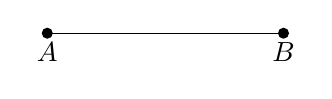
\begin{tikzpicture}
  \draw (0,0) -- (3,0);

  \fill (0,0) circle (2pt) node[below] {$A$};
  \fill (3,0) circle (2pt) node[below] {$B$};
\end{tikzpicture}

Časť priamky, ktorá vznikne tak, že úsečku \(AB\) predĺžime za bod \(B\), sa nazýva polpriamka. Budeme ju označovať \(\overrightarrow{AB}\). Bod \(A\) je začiatočný bod a bod \(B\) je vnútorný bod polpriamky \(\overrightarrow{AB}\).

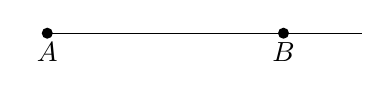
\begin{tikzpicture}
  \draw (0,0) -- (4,0);

  \fill (0,0) circle (2pt) node[below] {$A$};
  \fill (3,0) circle (2pt) node[below] {$B$};
\end{tikzpicture}

\section{Meranie}

Meranie je proces priraďovania veľkosti nejakej vlastnosti objektu. Výsledok merania je miera, ktorú vyjadrujeme pomocou čísla a jednotky. Merať môžeme veľkosť, množstvo, dĺžku, hmotnosť, čas, atď. Napríklad \(\SI{15}{\cm}\) je miera dĺžky. Pri meraní používame rôzne meradlá, napríklad pravítko, meter, váhu, hodiny alebo teplomer. Pomocou nich môžeme priradiť veľkosť odmeranej hodnote.

Podľa toho, čo meriame a akým meradlom meriame, zisťujeme veľkosť určitej veličiny v určitých jednotkách. Každá miera musí mať jednotku. Jednotka je dohodnutá veľkosť, pomocou ktorej meriame a vyjadrujeme veličiny. Bez jednotky by samotné číslo nedávalo zmysel. Preto musí každý výsledok merania byť číslo a k nej priradená jednotka. Vo väčšine krajín na svete (ako aj na Slovensku) sa používa dohodnutý súbor jednotiek nazývaný ako metrický systém. Iba tri štáty oficiálne metrický systém nepoužívajú: Mjanmarsko, USA a Libéria.

Meranie slúži na porovnávanie veľkostí. Veľkosti sú vyjadrené relatívne k nejakej dohodnutej hodnote. Napríklad \(1\) meter je určitá dĺžka, ku ktorej porovnávame odmeranú vzdialenosť. Dĺžka \(2\) metre je dvojnásobok dĺžky jedného metra. Miery s rovnakou jednotkou alebo k nim odvodeným jednotkám môžeme medzi sebou porovnávať na základe ich číselnej hodnoty.

Každé meradlo má svoju stupnicu. Stupnica je označená čiara alebo súbor značiek s číslami na meracom prístroji, podľa ktorých odčítavame nameranú hodnotu. Každé číslo určuje presnú mieru v jednotkách, ktoré sú zvyčajne napísané na meradle. Na stupnici nemusia byť číslom označené všetky možné miery, ktoré možno namerať. Rozdiel hodnôt medzi dvoma susednými značkami určuje, ako presne dokážeme merať. Každá stupnica má určitý merací rozsah. Merací rozsah stupnice je rozsah hodnôt od najmenšej po najväčšiu hodnotu, ktorú môžeme daným meradlom zmerať.

Meradlo môže mať iba konečný počet značiek, preto pri meraní musíme počítať aj s odchýlkou merania. Odchýlka merania je rozdiel medzi nameranou hodnotou a skutočnou alebo správnou hodnotou. Vzniká vtedy, keď nameraná hodnota \enquote{spadá} medzi dve značky. V takom prípade sa za nameranú hodnotu považuje tá značka, ktorá je bližšie k skutočnej hodnote. Odchýlku merania je možné vyčísliť. Odchýlka merania je vždy polovica rozdielu medzi dvoma susednými značkami. Napríklad ak je rozdiel susedných značiek \(\SI{1}{\cm}\), odchýlka merania je \(\pm \SI{5}{\mm}\). To znamená, že skutočná hodnota je niekde v rozmedzí \(-\SI{5}{\mm}\) až \(+\SI{5}{\mm}\) od nameranej hodnoty.

\begin{figure}[H]
  \centering
  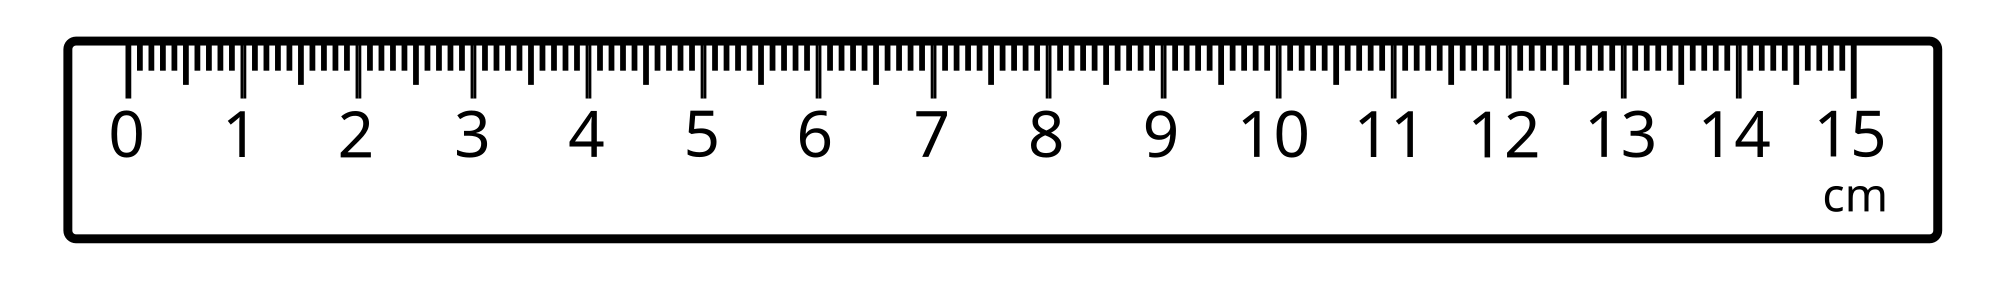
\includegraphics[width=1\textwidth]{Meter.png}
  \caption{Meradlo dĺžky s rozsahom \(\SI{0}{\cm}\) až \(\SI{15}{\cm}\), rozdielom medzi susednými dielikmi \(\SI{1}{\mm}\) a odchýlkou merania \(\pm \SI{0,5}{\mm}\).}
\end{figure}

\subsection{Meranie dĺžky}

Dĺžka je miera vzdialenosti medzi dvoma bodmi. Vzdialenosť udáva, koľko priestoru je medzi týmito bodmi. Základnou jednotkou dĺžky je meter (m). Menšie jednotky dĺžky sú decimeter (dm), centimeter (cm), milimeter (mm), väčšou jednotkou je kilometer (km). Medzi jednotkami dĺžky platia tieto vzťahy:

\noindent
\begin{tabularx}{\textwidth}{@{}XXXX@{}}
  \[
  \begin{aligned}
    \SI{1}{\km} &= \SI{1 000}{\m}, \\
    \SI{1}{\km} &= \SI{10 000}{\dm}, \\
    \SI{1}{\km} &= \SI{100 000}{\cm}, \\
    \SI{1}{\km} &= \SI{1000 000}{\mm},
  \end{aligned}
  \]
  &
  \[
  \begin{aligned}
    \SI{1}{\m} &= \SI{10}{\dm}, \\
    \SI{1}{\m} &= \SI{100}{\cm}, \\
    \SI{1}{\m} &= \SI{1000}{\mm},
  \end{aligned}
  \]
  &
  \[
  \begin{aligned}
    \SI{1}{\dm} &= \SI{10}{\cm}, \\
    \SI{1}{\dm} &= \SI{100}{\mm},
  \end{aligned}
  \]
  &
  \[
  \begin{aligned}
    \SI{1}{\cm} &= \SI{10}{\mm}.
  \end{aligned}
  \]
  \\
\end{tabularx}

\end{document}